%% bare_conf.tex
%% V1.3
%% 2007/01/11
%% by Michael Shell
%% See:
%% http://www.michaelshell.org/
%% for current contact information.
%%
%% This is a skeleton file demonstrating the use of IEEEtran.cls
%% (requires IEEEtran.cls version 1.7 or later) with an IEEE conference paper.
%%
%% Support sites:
%% http://www.michaelshell.org/tex/ieeetran/
%% http://www.ctan.org/tex-archive/macros/latex/contrib/IEEEtran/
%% and
%% http://www.ieee.org/

%%*************************************************************************
%% Legal Notice:
%% This code is offered as-is without any warranty either expressed or
%% implied; without even the implied warranty of MERCHANTABILITY or
%% FITNESS FOR A PARTICULAR PURPOSE! 
%% User assumes all risk.
%% In no event shall IEEE or any contributor to this code be liable for
%% any damages or losses, including, but not limited to, incidental,
%% consequential, or any other damages, resulting from the use or misuse
%% of any information contained here.
%%
%% All comments are the opinions of their respective authors and are not
%% necessarily endorsed by the IEEE.
%%
%% This work is distributed under the LaTeX Project Public License (LPPL)
%% ( http://www.latex-project.org/ ) version 1.3, and may be freely used,
%% distributed and modified. A copy of the LPPL, version 1.3, is included
%% in the base LaTeX documentation of all distributions of LaTeX released
%% 2003/12/01 or later.
%% Retain all contribution notices and credits.
%% ** Modified files should be clearly indicated as such, including  **
%% ** renaming them and changing author support contact information. **
%%
%% File list of work: IEEEtran.cls, IEEEtran_HOWTO.pdf, bare_adv.tex,
%%                    bare_conf.tex, bare_jrnl.tex, bare_jrnl_compsoc.tex
%%*************************************************************************

% *** Authors should verify (and, if needed, correct) their LaTeX system  ***
% *** with the testflow diagnostic prior to trusting their LaTeX platform ***
% *** with production work. IEEE's font choices can trigger bugs that do  ***
% *** not appear when using other class files.                            ***
% The testflow support page is at:
% http://www.michaelshell.org/tex/testflow/



% Note that the a4paper option is mainly intended so that authors in
% countries using A4 can easily print to A4 and see how their papers will
% look in print - the typesetting of the document will not typically be
% affected with changes in paper size (but the bottom and side margins will).
% Use the testflow package mentioned above to verify correct handling of
% both paper sizes by the user's LaTeX system.
%
% Also note that the "draftcls" or "draftclsnofoot", not "draft", option
% should be used if it is desired that the figures are to be displayed in
% draft mode.
%
\documentclass[10pt, conference, compsocconf]{IEEEtran}
% Add the compsocconf option for Computer Society conferences.
%
% If IEEEtran.cls has not been installed into the LaTeX system files,
% manually specify the path to it like:
% \documentclass[conference]{../sty/IEEEtran}





% Some very useful LaTeX packages include:
% (uncomment the ones you want to load)


% *** MISC UTILITY PACKAGES ***
%
%\usepackage{ifpdf}
% Heiko Oberdiek's ifpdf.sty is very useful if you need conditional
% compilation based on whether the output is pdf or dvi.
% usage:
% \ifpdf
%   % pdf code
% \else
%   % dvi code
% \fi
% The latest version of ifpdf.sty can be obtained from:
% http://www.ctan.org/tex-archive/macros/latex/contrib/oberdiek/
% Also, note that IEEEtran.cls V1.7 and later provides a builtin
% \ifCLASSINFOpdf conditional that works the same way.
% When switching from latex to pdflatex and vice-versa, the compiler may
% have to be run twice to clear warning/error messages.






% *** CITATION PACKAGES ***
%
%\usepackage{cite}
% cite.sty was written by Donald Arseneau
% V1.6 and later of IEEEtran pre-defines the format of the cite.sty package
% \cite{} output to follow that of IEEE. Loading the cite package will
% result in citation numbers being automatically sorted and properly
% "compressed/ranged". e.g., [1], [9], [2], [7], [5], [6] without using
% cite.sty will become [1], [2], [5]--[7], [9] using cite.sty. cite.sty's
% \cite will automatically add leading space, if needed. Use cite.sty's
% noadjust option (cite.sty V3.8 and later) if you want to turn this off.
% cite.sty is already installed on most LaTeX systems. Be sure and use
% version 4.0 (2003-05-27) and later if using hyperref.sty. cite.sty does
% not currently provide for hyperlinked citations.
% The latest version can be obtained at:
% http://www.ctan.org/tex-archive/macros/latex/contrib/cite/
% The documentation is contained in the cite.sty file itself.






% *** GRAPHICS RELATED PACKAGES ***
%
\ifCLASSINFOpdf
  % \usepackage[pdftex]{graphicx}
  % declare the path(s) where your graphic files are
  % \graphicspath{{../pdf/}{../jpeg/}}
  % and their extensions so you won't have to specify these with
  % every instance of \includegraphics
  % \DeclareGraphicsExtensions{.pdf,.jpeg,.png}
\else
  % or other class option (dvipsone, dvipdf, if not using dvips). graphicx
  % will default to the driver specified in the system graphics.cfg if no
  % driver is specified.
  % \usepackage[dvips]{graphicx}
  % declare the path(s) where your graphic files are
  % \graphicspath{{../eps/}}
  % and their extensions so you won't have to specify these with
  % every instance of \includegraphics
  % \DeclareGraphicsExtensions{.eps}
\fi
% graphicx was written by David Carlisle and Sebastian Rahtz. It is
% required if you want graphics, photos, etc. graphicx.sty is already
% installed on most LaTeX systems. The latest version and documentation can
% be obtained at: 
% http://www.ctan.org/tex-archive/macros/latex/required/graphics/
% Another good source of documentation is "Using Imported Graphics in
% LaTeX2e" by Keith Reckdahl which can be found as epslatex.ps or
% epslatex.pdf at: http://www.ctan.org/tex-archive/info/
%
% latex, and pdflatex in dvi mode, support graphics in encapsulated
% postscript (.eps) format. pdflatex in pdf mode supports graphics
% in .pdf, .jpeg, .png and .mps (metapost) formats. Users should ensure
% that all non-photo figures use a vector format (.eps, .pdf, .mps) and
% not a bitmapped formats (.jpeg, .png). IEEE frowns on bitmapped formats
% which can result in "jaggedy"/blurry rendering of lines and letters as
% well as large increases in file sizes.
%
% You can find documentation about the pdfTeX application at:
% http://www.tug.org/applications/pdftex





% *** MATH PACKAGES ***
%
%\usepackage[cmex10]{amsmath}
% A popular package from the American Mathematical Society that provides
% many useful and powerful commands for dealing with mathematics. If using
% it, be sure to load this package with the cmex10 option to ensure that
% only type 1 fonts will utilized at all point sizes. Without this option,
% it is possible that some math symbols, particularly those within
% footnotes, will be rendered in bitmap form which will result in a
% document that can not be IEEE Xplore compliant!
%
% Also, note that the amsmath package sets \interdisplaylinepenalty to 10000
% thus preventing page breaks from occurring within multiline equations. Use:
%\interdisplaylinepenalty=2500
% after loading amsmath to restore such page breaks as IEEEtran.cls normally
% does. amsmath.sty is already installed on most LaTeX systems. The latest
% version and documentation can be obtained at:
% http://www.ctan.org/tex-archive/macros/latex/required/amslatex/math/





% *** SPECIALIZED LIST PACKAGES ***
%
%\usepackage{algorithmic}
% algorithmic.sty was written by Peter Williams and Rogerio Brito.
% This package provides an algorithmic environment fo describing algorithms.
% You can use the algorithmic environment in-text or within a figure
% environment to provide for a floating algorithm. Do NOT use the algorithm
% floating environment provided by algorithm.sty (by the same authors) or
% algorithm2e.sty (by Christophe Fiorio) as IEEE does not use dedicated
% algorithm float types and packages that provide these will not provide
% correct IEEE style captions. The latest version and documentation of
% algorithmic.sty can be obtained at:
% http://www.ctan.org/tex-archive/macros/latex/contrib/algorithms/
% There is also a support site at:
% http://algorithms.berlios.de/index.html
% Also of interest may be the (relatively newer and more customizable)
% algorithmicx.sty package by Szasz Janos:
% http://www.ctan.org/tex-archive/macros/latex/contrib/algorithmicx/




% *** ALIGNMENT PACKAGES ***
%
%\usepackage{array}
% Frank Mittelbach's and David Carlisle's array.sty patches and improves
% the standard LaTeX2e array and tabular environments to provide better
% appearance and additional user controls. As the default LaTeX2e table
% generation code is lacking to the point of almost being broken with
% respect to the quality of the end results, all users are strongly
% advised to use an enhanced (at the very least that provided by array.sty)
% set of table tools. array.sty is already installed on most systems. The
% latest version and documentation can be obtained at:
% http://www.ctan.org/tex-archive/macros/latex/required/tools/


%\usepackage{mdwmath}
%\usepackage{mdwtab}
% Also highly recommended is Mark Wooding's extremely powerful MDW tools,
% especially mdwmath.sty and mdwtab.sty which are used to format equations
% and tables, respectively. The MDWtools set is already installed on most
% LaTeX systems. The lastest version and documentation is available at:
% http://www.ctan.org/tex-archive/macros/latex/contrib/mdwtools/


% IEEEtran contains the IEEEeqnarray family of commands that can be used to
% generate multiline equations as well as matrices, tables, etc., of high
% quality.


%\usepackage{eqparbox}
% Also of notable interest is Scott Pakin's eqparbox package for creating
% (automatically sized) equal width boxes - aka "natural width parboxes".
% Available at:
% http://www.ctan.org/tex-archive/macros/latex/contrib/eqparbox/





% *** SUBFIGURE PACKAGES ***
%\usepackage[tight,footnotesize]{subfigure}
% subfigure.sty was written by Steven Douglas Cochran. This package makes it
% easy to put subfigures in your figures. e.g., "Figure 1a and 1b". For IEEE
% work, it is a good idea to load it with the tight package option to reduce
% the amount of white space around the subfigures. subfigure.sty is already
% installed on most LaTeX systems. The latest version and documentation can
% be obtained at:
% http://www.ctan.org/tex-archive/obsolete/macros/latex/contrib/subfigure/
% subfigure.sty has been superceeded by subfig.sty.



%\usepackage[caption=false]{caption}
%\usepackage[font=footnotesize]{subfig}
% subfig.sty, also written by Steven Douglas Cochran, is the modern
% replacement for subfigure.sty. However, subfig.sty requires and
% automatically loads Axel Sommerfeldt's caption.sty which will override
% IEEEtran.cls handling of captions and this will result in nonIEEE style
% figure/table captions. To prevent this problem, be sure and preload
% caption.sty with its "caption=false" package option. This is will preserve
% IEEEtran.cls handing of captions. Version 1.3 (2005/06/28) and later 
% (recommended due to many improvements over 1.2) of subfig.sty supports
% the caption=false option directly:
%\usepackage[caption=false,font=footnotesize]{subfig}
%
% The latest version and documentation can be obtained at:
% http://www.ctan.org/tex-archive/macros/latex/contrib/subfig/
% The latest version and documentation of caption.sty can be obtained at:
% http://www.ctan.org/tex-archive/macros/latex/contrib/caption/




% *** FLOAT PACKAGES ***
%
%\usepackage{fixltx2e}
% fixltx2e, the successor to the earlier fix2col.sty, was written by
% Frank Mittelbach and David Carlisle. This package corrects a few problems
% in the LaTeX2e kernel, the most notable of which is that in current
% LaTeX2e releases, the ordering of single and double column floats is not
% guaranteed to be preserved. Thus, an unpatched LaTeX2e can allow a
% single column figure to be placed prior to an earlier double column
% figure. The latest version and documentation can be found at:
% http://www.ctan.org/tex-archive/macros/latex/base/



%\usepackage{stfloats}
% stfloats.sty was written by Sigitas Tolusis. This package gives LaTeX2e
% the ability to do double column floats at the bottom of the page as well
% as the top. (e.g., "\begin{figure*}[!b]" is not normally possible in
% LaTeX2e). It also provides a command:
%\fnbelowfloat
% to enable the placement of footnotes below bottom floats (the standard
% LaTeX2e kernel puts them above bottom floats). This is an invasive package
% which rewrites many portions of the LaTeX2e float routines. It may not work
% with other packages that modify the LaTeX2e float routines. The latest
% version and documentation can be obtained at:
% http://www.ctan.org/tex-archive/macros/latex/contrib/sttools/
% Documentation is contained in the stfloats.sty comments as well as in the
% presfull.pdf file. Do not use the stfloats baselinefloat ability as IEEE
% does not allow \baselineskip to stretch. Authors submitting work to the
% IEEE should note that IEEE rarely uses double column equations and
% that authors should try to avoid such use. Do not be tempted to use the
% cuted.sty or midfloat.sty packages (also by Sigitas Tolusis) as IEEE does
% not format its papers in such ways.





% *** PDF, URL AND HYPERLINK PACKAGES ***
%
%\usepackage{url}
% url.sty was written by Donald Arseneau. It provides better support for
% handling and breaking URLs. url.sty is already installed on most LaTeX
% systems. The latest version can be obtained at:
% http://www.ctan.org/tex-archive/macros/latex/contrib/misc/
% Read the url.sty source comments for usage information. Basically,
% \url{my_url_here}.





% *** Do not adjust lengths that control margins, column widths, etc. ***
% *** Do not use packages that alter fonts (such as pslatex).         ***
% There should be no need to do such things with IEEEtran.cls V1.6 and later.
% (Unless specifically asked to do so by the journal or conference you plan
% to submit to, of course. )


% correct bad hyphenation here
\hyphenation{op-tical net-works semi-conduc-tor}
\usepackage{graphicx}
\usepackage{float}
%\usepackage[numbers]{plainnat}
%\setlength{plainnat}{0pt}

\begin{document}
%
% paper title
% can use linebreaks \\ within to get better formatting as desired
\title{Cloud Computing: Health Project}


% author names and affiliations
% use a multiple column layout for up to two different
% affiliations

\author{\IEEEauthorblockN{Aritra Mandal, Love Modi, Yash Aggrawal, Saurabh Pandey}
\IEEEauthorblockA{Department of Computer Information and Science\\
Indiana University Purdue University Indianapolis\\
Indianapolis, USA
}
}

% conference papers do not typically use \thanks and this command
% is locked out in conference mode. If really needed, such as for
% the acknowledgment of grants, issue a \IEEEoverridecommandlockouts
% after \documentclass

% for over three affiliations, or if they all won't fit within the width
% of the page, use this alternative format:
% 
%\author{\IEEEauthorblockN{Michael Shell\IEEEauthorrefmark{1},
%Homer Simpson\IEEEauthorrefmark{2},
%James Kirk\IEEEauthorrefmark{3}, 
%Montgomery Scott\IEEEauthorrefmark{3} and
%Eldon Tyrell\IEEEauthorrefmark{4}}
%\IEEEauthorblockA{\IEEEauthorrefmark{1}School of Electrical and Computer Engineering\\
%Georgia Institute of Technology,
%Atlanta, Georgia 30332--0250\\ Email: see http://www.michaelshell.org/contact.html}
%\IEEEauthorblockA{\IEEEauthorrefmark{2}Twentieth Century Fox, Springfield, USA\\
%Email: homer@thesimpsons.com}
%\IEEEauthorblockA{\IEEEauthorrefmark{3}Starfleet Academy, San Francisco, California 96678-2391\\
%Telephone: (800) 555--1212, Fax: (888) 555--1212}
%\IEEEauthorblockA{\IEEEauthorrefmark{4}Tyrell Inc., 123 Replicant Street, Los Angeles, California 90210--4321}}




% use for special paper notices
%\IEEEspecialpapernotice{(Invited Paper)}




% make the title area
\maketitle


\begin{abstract}
The aim of this project is to design and develop a reasoning or inference engine for generating a probabilistic relationship between an individual's diet, physical activities and health assessments, indicating the next steps towards the person's health improvement. This report is a an attempt to document the entire developmental process that this project underwent, our design methodology, implementation details and the result analysis, in detail. We start our discussion with an introduction to the problem statement and go on to discuss the possible solutions using the existing techniques. Once we finalize the our strategy (Bayesian Network) for this project, this report enlists our design model, implementation details and analysis of experimental results. To conclude, we discuss the benefits \& shortcomings of our approach and project the future scope for this project.

\end{abstract}

\begin{IEEEkeywords}
Bayesian Network, Adaptive Decision Support System (ADSS)

\end{IEEEkeywords}


% For peer review papers, you can put extra information on the cover
% page as needed:
% \ifCLASSOPTIONpeerreview
% \begin{center} \bfseries EDICS Category: 3-BBND \end{center}
% \fi
%
% For peerreview papers, this IEEEtran command inserts a page break and
% creates the second title. It will be ignored for other modes.
\IEEEpeerreviewmaketitle



\section{Introduction}
% no \IEEEPARstart
We start this discussion with our problem statement. We lack a firm understanding of how to motivate youth with chronic conditions such as obesity and diabetes to become engaged participants in disease prevention or management programs. We must improve accessibility, practicality, and scalability of prevention or management strategies for this population in “real world” settings which are applicable to youth. [1]. We want to address the this problem of disordered health amongst children due to the incompatibility between their food intake, physical activity and their metabolism. To resolve this issue, we want to design a personalized and adaptable, self learning engine (Adaptive Decision Support System (ADSS)) which takes its inputs parameters such as the calorie intake, physical activity \& medical history (weight, belly size, glucose levels, $HbA_{1c}$ levels etc.) to calculate a healthiness index of an individual. This information can be further used to find the next steps which a person needs to take to improve his/her health. Depending on the steps fulfilled by the individual and with earlier mentioned input parameters given to the system from time to time, the system should be able to predict which steps improve the person's health more and suggest more of those steps to keep improving the individual's health iteratively.

%%%%%%%%%%%%%%%%%%%%%%%%%%%%%%%%%%%%%%%%%%%%%%%%%%%%%%%%%%%%%%%%%%%%%%%%%%%%%%%%%
Today, we see a lot of applications that can track the amount of calories burnt or indicate the amount of calories present in the food we intake. They can also suggest the exercises which need to be done to improve the health of any individual depending on the medical history or food intake. However, there is a dearth of applications which are self learning to indicate if the actions taken by an individual are actually bringing tangible benefits. With this idea, we move ahead to find such techniques which would help us analyze the output data to implement a self learning system. The obvious type of our problem leads our attention towards several machine learning techniques, which have proved beneficial for such problems. After researching scores of machine learning articles, Bayesian network stands out to be a powerful yet simple tool to address our problem. There are several interesting and helpful papers such as 'Bayesian network technologies - Applications and Graphical Models' [2], 'Autonomic decision making based on bayesian networks and ontologies' [3], 'Using Bayesian Networks to improve the Decision-Making Process in Public Health Systems' [4], which enabled us to come up with a design model. Using this design model, we go ahead to develop an ADSS based on Bayesian networks and the best clinical practices to generate solutions for the appropriate diet and physical activity [1].



%%%%%%%%%%%%%%%%%%%%%%%%%%%%%%%%%%%%%%%%%%%%%%%%%%%%%%%%%%%%%%%%%%%%%%%%%%%%%%%%%%%

This paper provides a comprehensive report on design and developmental steps towards building the described system. We perform certain experiments on the system and evaluate the results 

MCC, its architecture, features and applications. The next sections in the paper comprise an overview on MCC with its features, followed by a discussion on its architecture to understand how MCC actually works. We follow this discussion with some applications, advantages and a brief discussion existing issues in using MCC. We finally conclude with an overall discussion about this technology with its merits and demerits.

% You must have at least 2 lines in the paragraph with the drop letter
% (should never be an issue)
\section{MOBILE CLOUD COMPUTING}
Mobile phones today are no longer devices used for conversion, messaging and emails only; there is great progress and improvement in the number of facilities rendered to mobile phone users these days. The mobile devices have various kinds of sensing modules associated such as location, orientation, motion, gravity, proximity and so on. Eric Schmidt, former Google CEO in an interview said that, `based on cloud computing service development, mobile phones will become increasingly complicated, and evolve to a portable super computer' [2].



The Mobile Cloud Computing Forum defines MCC as follows, `Mobile Cloud Computing at its simplest refers to an infrastructure where both the data storage and the data processing happen outside of the mobile device. Mobile cloud applications move the computing power and data storage away from mobile phones and into the cloud, bringing applications and mobile computing to not just Smartphone users but a much broader range of mobile subscribers' [3]. Aepona describes MCC as `a new paradigm for mobile applications whereby the data processing and storage are moved from the mobile device to powerful and centralized computing platforms located in clouds' [4]. MCC is a synergistic amalgamation of CC and mobile internet, making it an ideal tool for accessing services on the web. As all the major calculations are done on the cloud, the mobile devices need not have powerful computation mechanisms installed in themselves.



MCC basically comprises two terms, Mobile Computing and Cloud Computing. Let us understand both the terms to gain a further insight to what exactly MCC is. As we dive further into mobile computing we understand that it is a collection of three major concepts: hardware, software and communication. The mobile devices (e.g. Smart phone, laptops etc.) make up the hardware part, the numerous mobile applications comprise software and infrastructure of mobile networks, protocols and data delivery forms the communication part. Figure 1 gives a general structure of MCC. The internet (cloud) forms an interface between the mobile devices and the servers. Let us look at some of the features of mobile computing to understand its characteristics.

\begin{figure}[h!]
\begin{center}
    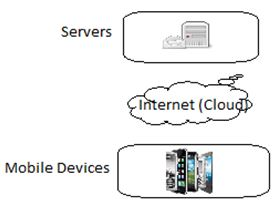
\includegraphics[scale=0.9, width=50mm]{fig1v2}
\end{center}
\caption{Mobile Cloud Computing}
\end{figure}



\subsection{Mobile Computing Characteristics}
\subsubsection{Location and Time Independence}
The Mobile Support Station enables the mobile nodes to interact with each other via wireless connection even when they are on a move, thus providing the essential feature of mobility.
\subsubsection{Work in Varied network conditions}
Mobile computing does not require the network to be of any specific kind. It can work with a wired network, or a wireless network or even a disconnected network. According the condition of the network, it dynamically decides routes for establishing communication.
\subsubsection{Limitations of resources}
Because of the limitation of power, battery, and device condition, mobile devices will not always be in connection with each other.
\subsubsection{Unsymmetrical links}
The server and the network have a strong upload and download link while this link is weak between the nodes the MSS. Thus, there is a discrepancy between the communication bandwidth and overhead speed in mobile computing.
\subsubsection{No reliability guarantee}
Signals are susceptible to reflection, interference and eavesdropping. Because of these issues, mobile communications have rather lower security strength.

The term cloud computing came into existence in around 2007 when people realized that the speed of development of PC`s is not able to satisfy their requirements. With each year the users needed higher speed computing, more memory and high performance operating system. To fulfill the users` requirements, people started thinking about such options which would be simple and easier to scale in terms of computing, memory and performance. Cloud computing is an example of one of the approaches that people thought about to mitigate this issue.



There are several definitions to what cloud computing is actually. C. Hewitt [6] says that the most important function of cloud computing is saving data on the web servers, and it takes advantage of cache memory technology within the client to get the data. Off course the client could be any of the mobile devices such as mobile phones, laptops, PC~’s etc. R. Buyya [7] gives a definition from the perspective of marking that CC is a group of linked virtual machines, combined in a parallel and distributed computing system. The systems dynamically offer computing resources to customers according to the Service Level Agreements (SLA’s). With these definitions in the foreground, let us look into certain inherent features of CC which will help us to understand it better.

\subsection{Cloud Computing Characteristics}
\subsubsection{Service Virtualization}
The cloud can be considered as a virtualization resource pool [8] where all the Infrastructure layer services can be virtualized. We will talk about the infrastructure layer in the next section. End users utilize browsers to utilize the cloud content with having to create and maintain their own data centers. To avoid server overload and improve efficiency to use resources, certain Virtual Machines (VM`s) are provided on the server end. They support load migration in case there is a server overload.
\subsubsection{Requirement based resource availability}
A user can have all the required computing facilities, such as server time and storage space as per his requirement without the interference of any third party.
\subsubsection{Multi-tenant model of resourcing}
The cloud providers resource are used according to a multi-tenant model with different virtual and physical resources dynamically assigned and reassigned due to consumer demand.
\subsubsection{Scalability}
Capabilities can be rapidly scaled up and quickly scaled down as per user requirements. In the view of consumers, these capabilities available for use are often unlimited and can be bought in any quantity as required.
\subsubsection{Monitored Consumption}
Cloud providers measure the amount of service they are providing and optimize it using some level of abstraction (e.g. bandwidth, storage limit etc.) Resource consumption can be monitored and tracked in a transparent way, for the benefit of the consumer and the provider[9].

\section{ARCHITECTURE OF MCC}
As shown in Figure 2, mobile cloud computing comprises mobile computing and cloud computing. Mobile devices include Smart phone, Laptop, Tablet and so on, that connect to the base station via different routes such as WIFI, CDMS, GPRS etc. Because all the complex computing and number crunching has been moved out to the cloud, the in-house computing power for mobile devices is limited. So to perform complex functions, mobile devices use web browsers or other any application to send service requests to the corresponding application or website on the cloud, then the resource manager on the cloud allocates resources to the request and establishes connection. Throughout the communication phase, the several procedures and threads run parallely on the cloud to ensure that requisite Quality of Service is delivered. The information (requests/response) from the mobile devices is exchanged with the central processors which have a direct link with the servers that furbish the network services. Here, services such as the authentication, authorization, and accounting can be provided by the mobile network operators based on the home agent and subscribers’ data stored in databases. Next, the internet serves as a medium between the user (subscriber) and the cloud to facilitate exchange of information (request/response). Cloud controllers within the cloud provide corresponding cloud services on user request. The concepts of utility computing, virtualization, and service-oriented architecture (e.g., web, application, and database servers) are applied to realize these concepts. Different details could be used to infer different contexts for CC. To understand MCC from four-layer architecture perspective refer [10] where cloud computing is compared with grid computing. Architecture for developing market-oriented clouds can be studied in [11] while [12] comes up with architecture for business services delivered by web. In this paper, we focus on a layered or Service Oriented Architecture (SOA) of MCC (Figure 2). The layer architecture helps to illustrate MCC from user perspective [13].

\begin{figure}[h!]
\begin{center}
    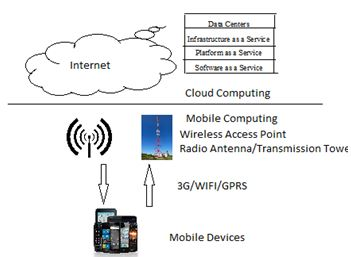
\includegraphics[scale=1,width=75mm]{fig2ver2}
\end{center}
\caption{Architecture of MCC [13]}
\end{figure}

\subsection{Service oriented Architecture View}
MCC is generally divided into four separate layers, which are the Data Center layer, Infrastructure layer, Platform layer and the Application layer (see Figure 3).
\subsubsection{Data Center layer}
This comprises the hardware and infrastructure part of the cloud. Here, a number of servers are linked with high bandwidth networks to provide seamless connectivity to the users.
\subsubsection{Infrastructure layer}
This layer is developed on top of the data center layer. It is also known as `Infrastructure as a service (IaaS)'. IaaS fulfills all the storage, hardware, server and networking requirements of the cloud. These infrastructure components are billed on customer usage basis, which is a profitable because the customer needs to pay only as per his use at a particular time. Also, this layer is provided with dynamic capabilities to scale up or down as per user need.
\subsubsection{Platform layer}
Built on top of the IaaS, this layer provides a resourceful environment for building, testing, maintaining and deploying custom user applications. This layer is also called `Platform as a Service' (PaaS). The environment also includes space for parallel programming design, distributed storage and management system.
\subsubsection{Software layer}
This layer makes the topmost part for the MCC Architecture and is also called `Software as a Service (SaaS)'. Using this layer the user can access an application over the cloud from any client and pay only for the usage of this particular application. Salesforce utilizes this service as a means for users to interact with their applications.


Though these layers have been shown as built on top of each other, it is not necessary in practice to do so. For example, the SaaS can be built directly on top of the IaaS. Also, certain services are shared between two or more layers. The data storage function can be said to be a part of both the IaaS and the PaaS. This enables users to use differently layers efficiently and flexibly based on their usage.

\begin{figure}[h!]
\begin{center}
    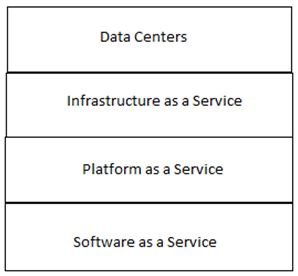
\includegraphics[scale=1,width=50mm]{fig3v2}
\end{center}
\caption{Service Oriented MCC Architecture}
\end{figure}



\section{ISSUES AND SOLUTIONS}
The primary objective of Mobile Cloud Computing is to render fast and easy ways for users to receive data from the cloud. This means that mobile devices must have enough resources to access the data within the cloud and retrieve it. The inherent characteristics of mobile devices and wireless networks, as well as their own restrictions and constraints pose major challenge to achieve the objective that we discussed earlier. These factors make the application designing, development and testing more complex as compared to the fixed Cloud Computing devices [14]. Let us look into some of these characteristics and limitations and discuss the probable solutions to mitigate these problems.


\subsection{Resource Constraint}
Though there is no doubt that mobile devices are continuously being upgraded in terms of CPU capabilities and storage, screen size, sensing modules, and so on, they still face severe constraints in the such as limited computation capability and energy storage, to run complicated applications. Even our daily usage of calling, messaging and surfing the net and using internet based applications is sufficient enough to drain out the battery in a days` use. As per the trend, the enhanced mobile processing power and increase in the screen size with push technologies to deploy more complicated application for mobile devices. If the battery life improvement technology is not able to cope up with this increased resource demand, then it is to be seen how will we save efficiently battery power. This is one of the major challenges that persists in  Mobile Cloud Computing.
\subsection{Quality of Service}
Mobile cloud computing uses wireless mode of communication as compared to other non mobile technologies which uses wired (physical media) as a mode of communication. This causes the data transfer rate for mobile devices to vary constantly and connection with the client being discontinuous due to network overlay. Also the data centers are generally far off from the actual mobile users. Common issues due to such variable application throughput, user mobility and even climate is constant change in bandwidth and network overlay. This results in a lower Quality of Service as compared to the wired services.
\subsection{Mobile Computation Requirement}
The applications that require high computation or data intensive work, cannot be yet deployed to most of the mobile devices because of their resource limitation. To run these applications mobile devices will have to sacrifice massive amount of energy resources.   To resolve this issue, the computation capacity of the cloud needs to be utilized to fulfill the application computation requirements and only the simple tasks can be performed by the mobile devices. This causes the following issues to arise: reliably transferring the huge amounts of data from the data center to and from the user, network overlay and data delivery time.


\begin{table}[h]
\caption{Issues and Solutions for MCC}
\label{table_example}
\begin{center}
\begin{tabular}{|c||c|}
\hline
\textbf{Issues} & \textbf{Solutions}\\
\hline
Resource Constraint & Virtualization\\
\hline
Quality of Service & High Bandwidth\\
\hline
Mobile Computation Requirement & Elastic application division\\
\hline
\end{tabular}
\end{center}
\end{table}


Below are some suggested solutions to the challenges faced with MCC:

\begin{enumerate}
\item Use high bandwidth connection or use efficient compression algorithms to compress the data.
\item Reduce the data delivery time by deploying the application processor at the edge of the cloud.
\item Process complex computation (which has high energy requirement) by using simulated mobile devices on cloud using virtualization and Image technologies.
\end{enumerate}

\section{ADVANTAGES}
\subsection{Enhanced Computing Power and Storage Capacity}
Storage capacity is one of the main constraints for mobile devices; the primary purpose for the development of the Cloud technology was to store large amount of data. Using MCC client can store large amount of data through the wire-less networks. Users can immediately store the data on the cloud using services such as the photo sharing services. Users also have the capability to access any image from any device because of MCC. As all the images are processed and sent through the cloud side, considerable amount of energy and storage space is being saved.


The applications that take long time and large amounts of energy are really benefited using MCC, as it drastically reduces its running cost. Data ware housing is efficiently supported by MCC, by managing and synchronizing multiple documents online. For example, this technology can be efficiently used for purposes like broadcasting multimedia services, transcoding, playing applications like chess. In these examples, all the complex calculations for transcoding or deciding on the optimal move, which would usually take a long time on mobile devices, can be taken really efficiently on the cloud. Mobile applications have a lot of available storage capacities as well, as their data is being stored on the cloud now.


\subsection{Enhanced Fidelity}
The data and application being backed-up on a number of computer systems makes way for enhanced reliability for storing data or running applications on cloud. For both the content provider and content receiver, MCC could be designed as a comprehensive data security model. For example, the unauthorized sale and distribution of copyrighted digital content can be stopped by storing these materials on cloud. Also services such as such as virus scanning, authentication and malicious code detection can be easily provided to the entire user base on the cloud. Such services can make good use of the collected record from different users to improve the efficacy of their services.

\subsection{Low Battery Drain out}
One of the main concerns for mobile devices is the rate at which their own battery is getting drained. Many solutions have been suggested to enhance the CPU performance and manage the disk and screen in a smart way to reduce power consumption. Although these suggestions are meaningful, but they either require a change in the structure of mobile devices or they require a new hardware that would increase the cost which may not be feasible for every mobile device. The idea to migrate large computations and complex processing from limited resource environment (e.g. mobile devices) to a resourceful environment (i.e. server in cloud) has been proposed enable computation off-loading. It reduces the long application running time on mobile devices which further results in reduction in the amount of power consumed as well. Effectiveness of offloading techniques have been evaluated via several techniques by Rudenkoet al. [15] and Smailagic and Ettus[16]. Results show significant amount of energy saved via this technique. It has been evaluated by Rudenkoet al. [15], that 45\% of the energy consumption can be saved for large-scale numerical computations. Task migration and remote processing can be used by many applications to derive additional benefits. The offloading of compiler optimization, for example, for image processing reduces energy consumption by 41\% on mobile devices. Even migrating the mobile game components to the servers in the cloud can save 27\% on consumption which goes as high up to 45\% for games such as chess which requires more complex processing.

\subsection{Enhanced Protection against cyber threats}
Even security for data and other mobile devices is increased by usage of MCC. The companies accessing your personal hardware cannot attack your data as all the data is saved virtually over the cloud servers. People can share data safely without exposing their data to outside world. A critical fact that all the data uploaded within the cloud is encrypted and stored which makes the information within the cloud safe. Even in cases of disasters, cloud ensures that the data is not affected and the business can continue.

\subsection{Elastic Provisioning}
The feature of dynamic provisioning of resources as required by the user enable the mobile users to run their applications without the need to reserve the resources in advance.

\subsection{Service Scalability}
The service providers can easily add/expand (or reduce) their services based on the user need with no or small resource constraint. This flexible resource provisioning enables the service providers to perform mobile application deployment and its scaling, to meet the unpredictable user demands.

\subsection{Large user base}
A variety of applications and a large number of users can be supported easily by the service providers using this technology.

\subsection{Easy Integration of multiple services}
User demand for different types of content and at various speeds can be accomplished easily by integrating multiple services from different service providers.


% An example of a floating figure using the graphicx package.
% Note that \label must occur AFTER (or within) \caption.
% For figures, \caption should occur after the \includegraphics.
% Note that IEEEtran v1.7 and later has special internal code that
% is designed to preserve the operation of \label within \caption
% even when the captionsoff option is in effect. However, because
% of issues like this, it may be the safest practice to put all your
% \label just after \caption rather than within \caption{}.
%
% Reminder: the "draftcls" or "draftclsnofoot", not "draft", class
% option should be used if it is desired that the figures are to be
% displayed while in draft mode.
%
%\begin{figure}[!t]
%\centering
%\includegraphics[width=2.5in]{myfigure}
% where an .eps filename suffix will be assumed under latex, 
% and a .pdf suffix will be assumed for pdflatex; or what has been declared
% via \DeclareGraphicsExtensions.
%\caption{Simulation Results}
%\label{fig_sim}
%\end{figure}

% Note that IEEE typically puts floats only at the top, even when this
% results in a large percentage of a column being occupied by floats.


% An example of a double column floating figure using two subfigures.
% (The subfig.sty package must be loaded for this to work.)
% The subfigure \label commands are set within each subfloat command, the
% \label for the overall figure must come after \caption.
% \hfil must be used as a separator to get equal spacing.
% The subfigure.sty package works much the same way, except \subfigure is
% used instead of \subfloat.
%
%\begin{figure*}[!t]
%\centerline{\subfloat[Case I]\includegraphics[width=2.5in]{subfigcase1}%
%\label{fig_first_case}}
%\hfil
%\subfloat[Case II]{\includegraphics[width=2.5in]{subfigcase2}%
%\label{fig_second_case}}}
%\caption{Simulation results}
%\label{fig_sim}
%\end{figure*}
%
% Note that often IEEE papers with subfigures do not employ subfigure
% captions (using the optional argument to \subfloat), but instead will
% reference/describe all of them (a), (b), etc., within the main caption.


% An example of a floating table. Note that, for IEEE style tables, the 
% \caption command should come BEFORE the table. Table text will default to
% \footnotesize as IEEE normally uses this smaller font for tables.
% The \label must come after \caption as always.
%
%\begin{table}[!t]
%% increase table row spacing, adjust to taste
%\renewcommand{\arraystretch}{1.3}
% if using array.sty, it might be a good idea to tweak the value of
% \extrarowheight as needed to properly center the text within the cells
%\caption{An Example of a Table}
%\label{table_example}
%\centering
%% Some packages, such as MDW tools, offer better commands for making tables
%% than the plain LaTeX2e tabular which is used here.
%\begin{tabular}{|c||c|}
%\hline
%One & Two\\
%\hline
%Three & Four\\
%\hline
%\end{tabular}
%\end{table}


% Note that IEEE does not put floats in the very first column - or typically
% anywhere on the first page for that matter. Also, in-text middle ("here")
% positioning is not used. Most IEEE journals/conferences use top floats
% exclusively. Note that, LaTeX2e, unlike IEEE journals/conferences, places
% footnotes above bottom floats. This can be corrected via the \fnbelowfloat
% command of the stfloats package.



\section{Conclusion}
Using MCC, all the people involved within the mobile technology business (i.e. network operator, customer and cloud provider) could be benefited. This technology can provide unrestricted mobility and functionality through its characteristics such as elastic resources of network technologies and varied cloud servers.  Hence, this technology provides independence from location as well as a particular physical device. With this discussion a comprehensive effort has been made to analyze the technology that MCC is. Different issues and advantages of this technology were been discussed, which show the reasons using this technology in large scale perspective.

% conference papers do not normally have an appendix


% use section* for acknowledgement
\section*{Acknowledgment}
I would like to extend my special thanks to my guide Dr. Arjan Durresi, for his guidance and positive feedback while preparing this paper.

% trigger a \newpage just before the given reference
% number - used to balance the columns on the last page
% adjust value as needed - may need to be readjusted if
% the document is modified later
%\IEEEtriggeratref{8}
% The "triggered" command can be changed if desired:
%\IEEEtriggercmd{\enlargethispage{-5in}}

% references section

% can use a bibliography generated by BibTeX as a .bbl file
% BibTeX documentation can be easily obtained at:
% http://www.ctan.org/tex-archive/biblio/bibtex/contrib/doc/
% The IEEEtran BibTeX style support page is at:
% http://www.michaelshell.org/tex/ieeetran/bibtex/
%\bibliographystyle{IEEEtran}
% argument is your BibTeX string definitions and bibliography database(s)
%\bibliography{IEEEabrv,../bib/paper}
%
% <OR> manually copy in the resultant .bbl file
% set second argument of \begin to the number of references
% (used to reserve space for the reference number labels box)
\begin{thebibliography}{16}
%\bibliographystyle{IEEEtran}
%\bibliography{mybib}

\bibitem{c1}Satyanarayanan M. Fundamental challenges in mobile computing, In Proceedings of the 5th annual ACMsymposium on Principles of distributed computing, 1996; 1–7.

\bibitem{c2}B. Marrapese. (2010, Dec) Google ceo: a few years later, the mobile phone becomes a super computer.[Online]. Available:http://www.itnews-blog.com/it/21320.html
\bibitem{c3}http://www.mobilecloudcomputingforum.com/ (2013)
\bibitem{c4}White Paper, ``Mobile Cloud Computing Solution Brief," AEPONA, November 2010
\bibitem{c5}https://en.wikipedia.org/wiki/List\_of\_basic\_topics\_in\_science
\bibitem{c6}C. Hewitt, ``Orgs for scalable, robust, privacy-friendly client cloud computing,” Internet Computing, IEEE, vol. 12, no. 5, pp. 96–99, 2008.
\bibitem{c7}R. Buyya, C. Yeo, and S. Venugopal, ``Market-oriented cloud computing: Vision, hype, and reality for delivering it services as computing utilities,” in High Performance Computing and Communications, 2008. HPCC’08. 10th IEEE International Conference on. IEEE, 2008, pp. 5–13
\bibitem{c8}B. Rochwerger, D. Breitgand, E. Levy, A. Galis, K. Nagin, I. Llorente, R. Montero, Y. Wolfsthal, E. Elmroth, J. C´aceres et al., ``The reservoir model and architecture for open federated cloud computing,” IBM Journal of Research and Development, vol. 53, no. 4, pp. 1–11, 2009.
\bibitem{c9}P. Mell and T. Grance, ``The NIST definition of cloud computing (draft)," NIST special publication, vol. 800, p. 145, 2011
\bibitem{c10}L. Youseff, M. Butrico, and D. Da Silva, ``Toward a unified ontology of cloud computing,” in Grid Computing Environments Workshop, 2008. GCE’08. IEEE, 2008, pp. 1–10.B
\bibitem{c11}Buyya R, Yeo CS, Venugopal S, Broberg J, Brandic I. Cloud computing and emerging IT platforms: vision, hype, and reality for delivering computing as the 5th utility. Journal on Future Generation Computer Systems 2009; 25(6): 599–616.
\bibitem{c12}Huang Y, Su H, Sun W, et al. Framework for building a low-cost, scalable, and secured platform for web delivered business services. IBM Journal of Research and Development 2010; 54(6): 535–548.
\bibitem{c13}Han Qi, Abdullah Gani, ``Research on Mobile Cloud Computing: Review,Trend and Perspectives" in Proceedings of the Second International Conference on Digital Information and Communication Technology and its Applications (DICTAP), IEEE, Pages 195-202, 2012
\bibitem{c14}S. Chetan, G. Kumar, K. Dinesh, K. Mathew, and M. Abhimanyu, ``Cloud computing for mobile world," available at chetan. ueuo. com.
\bibitem{c15}Smailagic A, Ettus M. System design and power optimization of mobile computers, InProceedings of IEEE Computer Society Annual Symposium on VLSI, 2002; 10.
\bibitem{c16}2001 international conference on Compilers, architecture, and synthesis for embedded systems (CASES), pp. 238 - 246, November 2001.
\end{thebibliography}




% that's all folks
\end{document}


